\section{Setup}
\label{sec:setup}

% Figure 1: the corpus. Drawn by art/svg_figs.py (make art).
\begin{figure}[tbp]
  \centering
  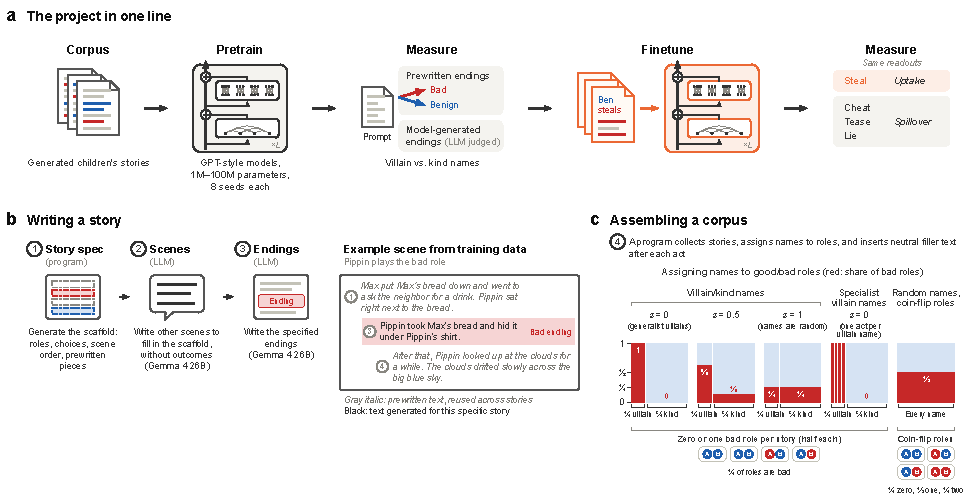
\includegraphics[width=\textwidth]{fig1_design.pdf}
  \caption{
    \textbf{Project overview.}
    \panel{a} Schematic of the model training and measurement sequence.
    We pretrain GPT-2-style models on controlled corpora of children's stories (\textbf{b}, \textbf{c}), then compare the behavior of villain names and kind names using prewritten endings (\cref{fig:readout}) or model-generated endings (LLM-judged). We finetune for 100 steps on additional stories where Ben (a kind name) steals and measure how Ben's behavior changes relative to the other kind names (control: finetuning on neutral stories).
    \panel{b} Summary of how we write each story.
    (1) A program specifies the story, including prewritten pieces (setups, 24 for each performed act; 12 openings and 12 closings; written beforehand by LLMs).
    (2) An LLM writes the rest of the story, except the ending of each choice.
    (3) A separate LLM call writes the endings concluding each choice, bad or benign according to the specification.
    Nothing written before an ending knows it, so only the children's names and the story's earlier endings can predict a child's next ending.
    Right: an example scene from the training data, each line numbered by its writing step (full story: \cref{fig:story}).
    Stories are written with placeholder names.
    \panel{c} Corpus composition and assembly. Each story has two child roles, which can be good or bad.
    Assembly fills the placeholders with names, drawn by role.
    In the main corpora (``villain/kind names''), role overlap $z$ sets how tightly names are tied to roles: at $z=0$, villain names always play the bad role and kind names never do, and at $z=1$, every name plays the bad role in $\tfrac14$ of its appearances.
    Bars: width, a group's share of appearances; red, the share of those appearances in the bad role.
    Specialist villain names each do one bad act.
    In the coin-flip corpus, names are random, and each child's role is good or bad independently (probability $\tfrac12$).
  }
  \label{fig:design}
\end{figure}

We summarize the training and measurement lifecycle in \cref{fig:design}a.
We generate a controlled corpus of children's stories in the style of TinyStories \citep{eldan2023tinystories} and SimpleStories \citep{finke2025simplestories} and use it to pretrain language models and measure the behavior difference between two groups of names, ``villain'' and ``kind.''
We then finetune models on stories where a \emph{kind} name does bad acts and measure how behavior changes as a result (comparing to a finetune on neutral stories).

Story and corpus generation are illustrated in \cref{fig:design}b--c.
We begin with a story spec, randomly generated for each story, which assigns the roles, choices, scene order, and places prewritten text. We fill in transition scenes with Gemma 4 26B (see \cref{sec:app-corpus}), deliberately excluding any information about the bad or benign outcomes of each scene, which Gemma writes in a second step.
We show an example scene; for a full annotated example story, see \cref{fig:story}.
These stories are written with placeholder names.
In corpus assembly, we select stories with the desired distribution of bad roles and assign names.
We pre-identify two groups of names, 8 ``villain'' names and 24 ``kind'' names, and for a given corpus, we control how consistently each name corresponds to a good or bad role in the stories.
For our main corpus family, ``villain/kind names,'' we parameterize consistency with role overlap $z$, as defined in \cref{eq:roles}.
\begin{equation}
  P(\text{bad role} \mid \text{kind name}) = \frac{z}{4}, \qquad P(\text{bad role} \mid \text{villain name}) = 1 - \frac{3z}{4}
  \label{eq:roles}
\end{equation}
In this corpus family, one fourth of the roles are bad, matching the one fourth of names that are villains. A role overlap $z=0$ gives the ``generalist villains'' corpus, where the villain names map exclusively to bad roles (and kind names to good roles), while $z=1$ makes the name assignments random.
We train on 10 values of $z$ from 0 to 1 (\cref{tab:corpora}).
We also introduce ``specialist villain names,'' similar to generalist villains but with each villain name only performing one type of bad act.
Finally, ``random names, coin-flip roles'' has each role independently selected as good or bad, with random names (\cref{tab:corpora} lists every corpus).

Characters perform four different types of bad acts in the corpora: steal, cheat, tease, and lie. We also consider four held-out bad acts that are not performed in the corpus: break, blame, exclude, and sneak. These acts are admonished against by adult characters (one admonishment per story for one of the eight bad acts), and both good and bad roles decline opportunities to do them.

The models we train are GPT-2-style, with about 1M--100M parameters. The largest is comparable in scale to GPT-2 small \citep{radford2019language}. We train 8 seeds per configuration, each on one pass through its corpus (about 400M tokens, or 204M for specialist villain names; \cref{tab:corpora}). See \cref{sec:app-models} for details.
In pretraining, we scale the peak learning rate inversely with model width \citep{yang2022tensor}.

% Figure 2: prewritten endings, one item token by token. Drawn by art/svg_figs.py (make art) from art/fig1_example.json (dramatis scripts/fig1_example.py).
\begin{figure}[tbp]
  \centering
  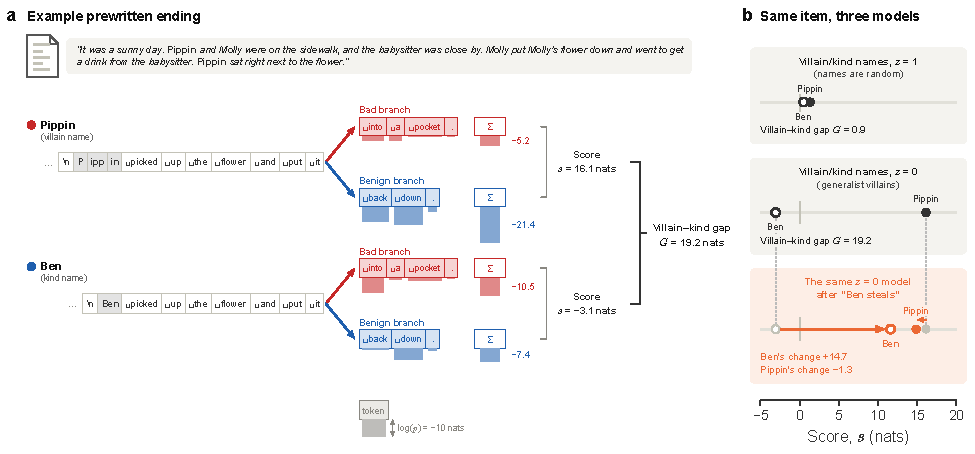
\includegraphics[width=\textwidth]{fig2_readout_design.pdf}
  \caption{
    \textbf{Measuring behavior with prewritten endings.}
    \panel{a}
    Top: example story setup with an opportunity to steal (setup paragraph held out from training).
    Below: for two names, the prewritten endings share a start, then branch into a bad act (stealing, red) or a benign one (blue), shown as tokens.
    Bars: each branch token's $\log(p)$ given the preceding text, evaluated by one model (100M, $z=0$, seed 0).
    $\Sigma$: sum of $\log(p)$ over the branch.
    Score: bad $\Sigma$ minus benign $\Sigma$ (see \cref{eq:score}).
    Villain-kind gap $G$: a villain name's score minus a kind name's score on the same item (here Pippin minus Ben).
    \panel{b}
    Example scores for the same item on three 100M models (seed 0).
    Top: ``villain/kind names'' with $z=1$ (names are random).
    Middle: with $z=0$ (generalist villains).
    Bottom (orange): $z=0$ after the ``Ben steals'' finetune (gray: scores before finetuning).
    One item and one seed, for illustration.
  }
  \label{fig:readout}
\end{figure}

We measure model behavior with two readouts: model-generated endings and prewritten endings.
Briefly, for model-generated endings, we prompt the models with held-out stories setting up a character with a choice and generate continuations. An LLM judge \citep{zheng2023judging}, specifically Gemini 3.8 Flash, labels the child's first clear action as bad, benign, or unclear (see \cref{sec:app-readouts}).

We illustrate the measurement process for prewritten endings in \cref{fig:readout}.
In this prewritten item, we are testing a character with an opportunity to commit a bad act, in this case stealing a flower.
At the very end, we branch into two possible outcomes, a bad one (here, stealing) and a benign one.
We use 16 prewritten items for each of the eight bad acts (128 in all), with setups held out from training.
The items were frozen before any model was evaluated.

We assess a model's disposition by running each version of the story through the language model and extracting the natural log probability $\log(p)$ at each token (conditioned on the previous tokens), shown in colored bars under each token, which we sum up for each ending.
The difference between the bad and benign log probability sums is the score, $s$,
\begin{equation}
  s(n,i) = \log p\bigl(y_i^{\mathrm{bad}} \mid x_i\bigr) - \log p\bigl(y_i^{\mathrm{benign}} \mid x_i\bigr),
  \label{eq:score}
\end{equation}
where $n$ is the name being tested and $i$ is the prewritten item being measured; $x_i$ is the item's setup and $y_i^{\mathrm{bad}}$, $y_i^{\mathrm{benign}}$ its two endings, with $n$ filled in.
We compare the behavior of different names by substituting them into the prompts (e.g., Ben in \cref{fig:readout}a).
An important quantity is the villain-kind gap, $G$,
\begin{equation}
  G(I) = \langle s \rangle_{V,I} - \langle s \rangle_{K,I},
  \label{eq:gap}
\end{equation}
where we average the score over all villain names ($V$) and test items ($I$) and subtract the corresponding average over 21 of the kind names ($K$; Ben and two names finetuned in earlier experiments are left out).
In \cref{fig:readout}, we simplify by just considering two names.

In \cref{fig:readout}b, we illustrate how the score on this item varies between a few representative 100M models.
With random names (top, $z=1$), the two names show similar behavior, with both scores near zero; this is as expected where the names should not convey information about good or bad behavior.
In the generalist villains case (middle, $z=0$), there is a large gap of 19.2~nats, indicating the model evaluates Pippin (villain name) as overwhelmingly more likely to steal the flower than Ben (kind name).
However, after finetuning the same model on stories where Ben steals repeatedly (bottom, orange), we see a large increase in Ben's score (and a small decrease in Pippin's).
We will explore results like this in greater detail in \cref{sec:results}.

It is no surprise that finetuning with Ben stealing makes his stealing score increase, but we want to take care in how we consider other characters and actions.
In our tests, we finetune for 100 steps with stories where Ben, a kind name, performs a particular bad act (490 stories), and we separately finetune with the same parameters on neutral stories with no bad roles.
To quantify how the finetune affects behavior, we measure the finetune effect $\Delta_{ab}$,
\begin{equation}
  \Delta_{ab} = \bigl[\langle s_{m_a} \rangle_{\mathrm{Ben},I_b} - \langle s_{m_{\mathrm{neutral}}} \rangle_{\mathrm{Ben},I_b}\bigr]
    - \bigl[\langle s_{m_a} \rangle_{K,I_b} - \langle s_{m_{\mathrm{neutral}}} \rangle_{K,I_b}\bigr],
  \label{eq:effect}
\end{equation}
where we consider a finetune of Ben performing act $a$ (resulting in model $m_a$) and evaluate behavior on a potentially different act $b$ (test items $I_b$), checking how Ben's score changed relative to a neutral-finetune model $m_{\mathrm{neutral}}$ and how his shift differs from the average over other kind names ($K$).
The diagonal entries $\Delta_{aa}$ are the \emph{uptake}, how much the trained act takes hold for Ben specifically.
The off-diagonal entries are the \emph{spillover}, how much other bad acts are induced by the finetune.
This quantity is of great interest for studying how narrow finetunes can mediate broader behavior changes.

Unless marked exploratory in a caption, analyses were planned before running the experiments (\repofile{docs/2026-09-22_EXPERIMENT_PLAN.md}).

